\chapter{Entorno de desarrollo}\label{chap:entorno}

Para el desarrollo del proyecto se ha hecho uso de una gran cantidad de herramientas y tecnologías que es importante ver para poder comprender mejor el modo de desarrollo.

\section{CMake}

CMake es una herramienta para la construcción de fichero Makefile. El mayor inconveniente que hay a la hora de utilizar ficheros Makefile es que es complicado mantenerlos y aún más crear versiones para diferentes sistemas operativos. Este último punto se debe a que puede variar sutilmente algunas de las reglas de para crear el fichero y que dependiendo del sistema operativo se puedan necesitar unas u otras librerías. Además, utilizando ficheros Makefile es complicado realizar comprobaciones sobre el sistema, com puedan ser comprobar si está o no instalada una biblioteca en concreto.

Existen varias soluciones para la generación de ficheros Makefile, entre ellas destaca GNU Autotools. Ésta es probablemente una de las herramientas más famosas en el mundo del software libre por ser la que se utiliza dentro del proyecto GNU. Desgraciadamente Autotools es una herramienta complicada de utilizar lo que nos hizo decantarnos por CMake.

CMake utiliza una sintaxis sencilla para definir las reglas de comprobación, asignación de dependencias y cualquier cosa que tenga que ver con el proceso de generación del proyecto.

Para instalar cmake en el sistema se ejecutará el siguiente comando:

\begin{verbatim}
$ sudo apt-get install cmake
\end{verbatim}

\section{Git}

Una parte muy importante de todo proyecto es la gestión de los ficheros que se están utilizando. En el caso de un proyecto software el control de los cambios es fundamental para evitar problemas.

Git es un sistema de control de versiones desarrollador por Linus Torvalds para el núcleo Linux. Sus principales características son:

\begin{itemize}
	\item Es un sistema distribuido, lo que evita la necesidad de disponer siempre de un servidor central al que enviar los cambios, como sucede con otros sistemas como CVS o Subversion.
	
	\item Facilita la creación de ramas (\emph{branch}) de desarrollo y la fusión de éstas (\emph{merge}) cuando es necesario de forma rápida y sencilla.
	
	\item Facilita disponer de copias de seguridad distribuyéndolas entre varios equipos, al menos en el uso que se ha dado para este proyecto final de carrera.
\end{itemize}

Para poder utilizar git solo hace falta instalarlo ejecutando el siguiente comando:

\begin{verbatim}
$ sudo apt-get install git-core
\end{verbatim}

Durante el desarrollo del proyecto se ha utilizado varias ramas para controlar las distintas partes. Concretamente se ha utilizado:

\begin{description}
	\item[master] Mantiene el código que ha se ha comprobado que funciona correctamente. No se puede incorporar nada a esta rama directamente, sino que hay que desarrollar primero en otra rama, comprobar correcto funcionamiento de los cambios y luego se realiza la mezcla de los cambios con master.
	
	\item[ldopen] En esta rama se realizaron los cambios para soportar plugins. La nomenclatura de ldopen proviene de la llamda a sistema utilizada para poder desarrollar esta funcionalidad.
	
	\item[nuevaweb] Aquí se encuentra todo el código de pruebas del nuevo controlador desarrollado así como cambios sobre los agentes para soportar la nueva arquitectura.
	
	\item[fixcompiling] Cambios realizados para que la compilación en el sistema operativo Mac OS X funcionara correctamente.
\end{description}

\section{Apache}

Para poder hacer uso del controlador es necesario disponer de un servidor web con soporte de PHP. En este caso se ha utilizado el servidor web Apache en su versión 2 por ser el más popular, disponer de una abundante documentación y ser software libre.

Cualquier distribución de GNU/Linux puede instalar este servidor web con unos pocos clicks de ratón o en su defecto un único comando. en el caso de las distribuciones basadas en Debian solo hace falta ejecutar el siguiente comando:

\begin{verbatim}
$ sudo apt-get install apache2
\end{verbatim}

\section{Redmine}

Redmine es un gestor de proyectos realizado en Ruby on Rails. Permite la asignación de tareas, calendarios, documentación y otras muchas funcionalidades más a través de plugins. Como la mayoría de las herramientas utilizadas es software libre.

Esta herramienta ha sido de utilidad para poder controlar los problemas que han ido surgiendo y que no quedaran pendientes.

La instalación de redmine es probablemente de las más complicadas de todas las herramientas utilizadas en este proyecto. Para instalar esta herramienta se ha tenido que seguir los siguientes pasos:

\begin{itemize}
	 \item Instalación de ruby, rails y rake:
	 \begin{verbatim}
	 $ sudo apt-get install ruby rails rake
	 \end{verbatim}
	 
	 \item Instalación del módulo passenger para apache\footnote{Passenger dispone de paquetes para algunas distribuciones. Por desgracia, la distribución que utilizaba el servidor de Redmine no disponía de dichos paquetes}:
	 \begin{verbatim}
	 $ sudo gem install passenger
	 $ sudo passenger-install-apache2-module
	 \end{verbatim}
\end{itemize}

\section{CUDA}

Como no, se ha hecho uso de las herramientas de NVIDIA para compilar el proyecto. El \emph{framework} CUDA trae las bibliotecas básicas necesarias para poder comunicarse con la tarjeta gráfica y las herramientas de compilación.

Para poder utilizar CUDA hay que instalar previamente los controladores de la tarjeta gráfica adecuados ya que los controladores que vienen por defecto solo permiten funciones gráficas.

Para desarrollar el proyecto se ha hecho uso de la versión 2.3 de CUDA que puede encontrarse en \url{http://developer.nvidia.com/object/cuda_3_2_downloads.html}. Desde esta página se pueden descargar tanto los controladores para el sistema operativo como las herramientas necesarias para desarrollar en CUDA.

Es importante comprobar antes de utilizar CUDA si la tarjeta gráfica que tiene el equipo es compatible.

Para instalar CUDA en linux se necesita instalar primero el controlador de la tarjeta gráfica. Este controlador requiere las cabeceras del núcleo Linux para poder compilarse. Por este motivo hay que asegurarse de que ya se encuentre instaladas y en caso contraro se puden instalar con el siguiente comando:

\begin{verbatim}
$ sudo apt-get install linux-headers-generic
\end{verbatim}

Por desgracia no se ofrecen paquetes adaptados a cada distribución por lo que hay que utilizar el instalador que ofrece NVIDIA:

\begin{verbatim}
$ wget http://developer.download.nvidia.com/compute/cuda/
3_2_prod/drivers/devdriver_3.2_linux_32_260.19.26.run
$ sudo sh ./devdriver_3.2_linux_32_260.19.26.run
\end{verbatim}

Tras este paso solo hay que siguir las indicaciones del instalador.

Hay ocasiones en las que el instalador de los controladores de NVIDIA fallan y no crean los dispositivos necesarios en /dev, por lo que hay que crearlos a mano. Para ello se puede utilizar las siguiente llamdas en línea de comando:

\begin{verbatim}
$ for i in $(seq 0 9); do sudo mknod /dev/nvidia${i} c 195 ${i}; done
$ sudo mknod /dev/nvidiactl c 195 255
\end{verbatim}

Una vez instalado el controlador de CUDA se puede proceder a instalar las herramientas. Éstas utilizan su propio instalador, pero está adaptado a distintas distribuciones, por lo que hay que elegir el más adecuado:

\begin{verbatim}
$ wget http://developer.download.nvidia.com/compute/cuda/
3_2_prod/toolkit/cudatoolkit_3.2.16_linux_64_ubuntu10.04.run
$ sudo sh ./cudatoolkit_3.2.16_linux_64_ubuntu10.04.run
\end{verbatim}

Es recomendable instalar las herramientas en los directorios que nos indique como predeterminados (generalmente /usr/local/cuda).

\section{g++}

El compilador de GNU es probablemente uno de los más utilizados hoy día en el mundo del software libre. Este compilador dispone de herramientas para compilar una gran cantidad de lenguajes distintos como C, C++, Objective-C, Pascal y muchos más. Es el compilador que traen todas las distribuciones GNU/Linux en la actualidad y hasta sistemas operativos como Mac OS X lo utilizan.

La mayor parte del código empleado en el proyecto está escrito en C++ por lo que se ha necesitado hacer uso del compilador de C++ que de GNU, principalmente por ser el más sencillo de instalar.

Para asegurarnos que al instalar el compilador g++ se instalen todas las dependencias que necesitamos podemos ejecutar la siguiente orden:

\begin{verbatim}
$ sudo apt-get install build-essential g++
\end{verbatim}

El paquete build-essential se encarga de instalar todas las herramientas y bibliotecas de compilación básicas. Luego le indicamos que se asegure de instalar g++.

\section{PHP}

PHP es un lenguaje de programación web muy extendido gracias a que es gratuito y libre. Tiene una sintaxis sencilla fuertemente basada en C y es muy fácil de aprender.

Es muy habitual hablar de instalaciones LAMP, que son aquellas que hacen uso de Linux, Apache, MySQL y PHP y que son ampliamentes utilizadas en internet por gran número de servicios de alojamiento por su bajo coste y facilidad de instalación y configuración.

Al ser un lenguaje muy extendido se ha utilizado para la creación del nuevo controlador de DHC. El anterior controlador también hacía uso de PHP pero cuando se planteó crear uno nuevo se barajaron soluciones basadas en Ruby y Groovy. Estas soluciones fueron descartadas por ser algo más complicadas de configurar. Para ser más precisos, Ruby requiere que se instalen modulos especiales para Apache y hay que revisar muy bien la configuración. En el caso de Groovy se necesita un servidor Apache Tomcat basado en java que puede suponer una gran sobrecarga para el sistema.

Para instalar PHP e integrar éste con Apache solo hace falta ejecutar el siguiente comando en cualquier distribución basada en Debian:

\begin{verbatim}
$ sudo apt-get install php5
\end{verbatim}

\section{CakePHP}

CakePHP es un \emph{framework} de desarrollo web que hace uso del lenguaje de programación PHP y el patrón de diseño MVC. Con CakePHP se pueden hacer aplicaciones fácilmente sin tener que preocuparse de cosas como el acceso a base de datos o el control de flujo a través de la aplicación.

Gracias al uso de CakePHP se ha podido centrar la atención del controlador más en las tareas propias del mismo. De este modo ahora no hay que preocuparse de como hacer el acceso a la base de datos o incluso el tipo de base de datos que se está utilizando.

Para utilizar CakePHP solo hace falta descargarlo y descromprimirlo en un directorio. Éste ya dispone de una estructura básisca de directorios para utilizar directamente en un proyecto. Para este proyecto los directorios más importantes son:

\begin{description}
	\item[app/controllers] Almacena los controladores de la aplicación. Estos controladores se encargan de la lógica de negocio.
	
	\item[app/views] Representan las salidas que producirá la aplicación.
	
	\item[app/models] Describe la estructura de la base de datos (las tablas y sus relaciones).

	\item[app/config] Tiene la configuración de qué motor de base de datos hay que utilizar y la configuración de la misma. Por otra parte se ha almacenado aquí el script para generar las tablas en esta base de datos.
\end{description}

\section{MySQL}

MySQL es uno de los motores de base de datos libres más extendidos de internet. La principal razón de ésto es que es fácil de administrar y que históricamente siempre ha sido una base de datos muy rápida, lo que suponía una ventaja para las aplicaciones web con una alta carga de peticiones.

El controlador de DHC hace uso de bases de datos para almacenar la información de las tareas que se están ejecutando y las estadísticas de las mismas.

Su instalación es tan sencilla como ejecutar:

\begin{verbatim}
$ sudo apt-get install mysql-server
\end{verbatim}

\section{Gimp}

Gimp es una herramienta de retoque fotográfico de una gran calidad y que desde hace muchos años se la considera el Photoshop del software libre.

Para las imágenes utilizadas en la web se ha utilizado Gimp por ser una herramienta potente y relativamente sencilla de utilizar.

Para su instalación se ha utilizado:

\begin{verbatim}
$ sudo apt-get intall gimp
\end{verbatim}

\section{\LaTeX}

Es una de las herramientas más extendidas para la creación de textos científicos. \LaTeX son un conjunto de reglas para la herramienta \TeX creada por Donald E. Knuth. Su diseño está pensado para no tener que prestar demasiada atención a detalles de presentación para centrar el esfuerzo en el contenido. Es muy parecido a lo que ahora se hace en web con HTML+CSS.

La memoria de este proyecto final de carrera ha sido escrito utilizando \LaTeX por las ventajas que ofrece frente a otros sistemas como Microsoft Word o LibreOffice. Entre estas ventajas podemos destacar que al almacenar solo ficheros de texto es más sencillo realizar un control de versiones sobre las modificaciones, lo que resulta más complicado utilizando ficheros binarios.

Para instalar el compilador de \LaTeX en el sistema hay que ejecutar:

\begin{verbatim}
$ sudo apt-get install texlive-latex-extra
\end{verbatim}

\section{GnuPlot}

GnuPlot es una herramienta para la generación de gráficas de funciones. Ha sido utilizada para la gráfica de la distribución de la paradoja del cumpleaños.

Esta herramienta es muy útil cuando se necesita hacer gráficas de datos y no se tiene un sistema muy potente ya que requiere de poca memoria. Un ejemplo de ello es cuando se tienes grandes tablas de datos en MS Office lo que hace que tarde en generar gráficas o incluso manejar los datos.

En este caso se ha creado un script de GnuPlot que ha sido integrado dentro del sistema de compilación automático de CMake para generar un PDF y poder ser incrustado en el documento \LaTeX.

Para instalar GnuPlot solo hace falta utilizar la siguiente orden en el sistema:

\begin{verbatim}
$ sudo apt-get install gnuplot
\end{verbatim}

\section{LibreOffice}

LibreOffice es una herramienta que ha nacido a partir del código de OpenOffice.org. Su creación viene motivada a que los desarrolladores de OpenOffice.org estaban a disgusto con las políticas empresariales de Oracle.

Todas los diagramas que aparecen en la memoria ha sido realizadas con la aplicación de dibujo de LibreOffice.

LibreOffice puede ser descargado desde su página web en \url{http://www.libreoffice.org/download/}.

\section{UML}

UML, siglas de \emph{Unified Modeling Language}, es un lenguaje gráfico para modelar software ampliamente utilizando en el mundo de la programación orientada a objetos.

Algunos de los diagramas expuestos en la memoria hacen uso de dicho lenguaje. Concretamente se ha hecho uso de diagramas de clases y de secuencia. El primero permite expresar de forma gráfica los elementos que formar todo, o una parte, de un programa, pero sin entrar al detalle de como deben comportarse. Los diagramas de secuencia representan un caso de funcionamiento concreto y son útiles para poder mostrar cómo actúa una parte del proyecto.

\section{Debian y Ubuntu}

Debian es una de las distribuciones de Linux más antiguas y su filosofía es utilizar solo software libre. Una de los puntos más importantes a destacar sobre esta distribución es que está mantenida enteramente por voluntarios y que tiene uno de los mayores repositorios de aplicaciones de todas las ditribuciones existentes.

Debian posé muchas distribuciones derivadas que sobre ésta añaden paquetes y/o hacen cambios de configuración. Una de estas distribuciones, y probablemente la ditribución más famosa actualmente, es Ubuntu.

Para descargar Debian se puede ir a \url{http://www.debian.org/distrib/} y Ubuntu se puede obtener de \url{http://www.ubuntu.com/desktop/get-ubuntu/download}.

\section{SLOCCount}

SLOCCount es una herramienta para contar número de líneas de código de proyectos software. Tras una ejecución de esta herramienta sobre un directorio con software ofrece estadísticas del número de líneas total y cómo se distribuyen entre los distintos lenguajes de programación utilizados.

Además de lo anterior, SLOCCount trata de hacer una estimación del coste del código comprobado utilizando el modelo COCOMO.

Para poder utilizar esta herramienta hay que instalarla previamente con el siguiente comando:

\begin{verbatim}
$ sudo apt-get install sloccount
\end{verbatim}

\section{Organización del entorno de trabajo}

Para realizar el proyecto se ha utilizado, a parte de las herramientas anteriormente mencionadas, una serie de equipos organizados del siguienet modo:

\begin{description}
	\item[Servidor web] Se dispone de un servidor privado virtual que tiene instalado Apache, Git, Redmine, PHP y la versión de pruebas del controlador de DHC.
	
	Este servidor ha sido subcontratado para garantizar un buen funcionamiento del servicio ya que la red de la universidad no ofrece garantías suficientes de estabilidad. Además, el uso de un servidor privado virtual ofrece la posibilidad de instalar todas aquellas herramientas que sean necesarias.
	
	\item[Equipos de desarrollo] Puede ser cualquier equipo desde el que puede escribirse código fuente. Se han utilizado dos ordenadores para este propósito uno con Mac OS X y el otro con Kubuntu 10.10.
	
	Desde estos equipos se realizan constantes peticiones de \emph{pull} y \emph{push} a git para mantener siempre una copia actualizada de los cambios.
	
	\item[Equipo de ejecución] Este equipo se encuentra instalado en el laboratorio de Evalues en el Parque Cientifico-Tecnológico de Leganés. Dispone de una 2 microprocesadores AMD Opteron de 4 núcleos cada uno, 8 GB de RAM y una NVIDIA Tesla S1070.
	
	Tanto la unidad Tesla como el equipo que la controla pueden montarse en un \emph{rack} de ordenadores.
	
	Para ejecutar las pruebas este ordenador hace peticiones de \emph{pull} al git para obtener las versiones más actuales del código.
\end{description}

Para comprender mejor como interactúan entre sí los distintos se puede consultar la figura~\ref{fig:entorno_trabajo}.

\begin{figure}
	\centering
	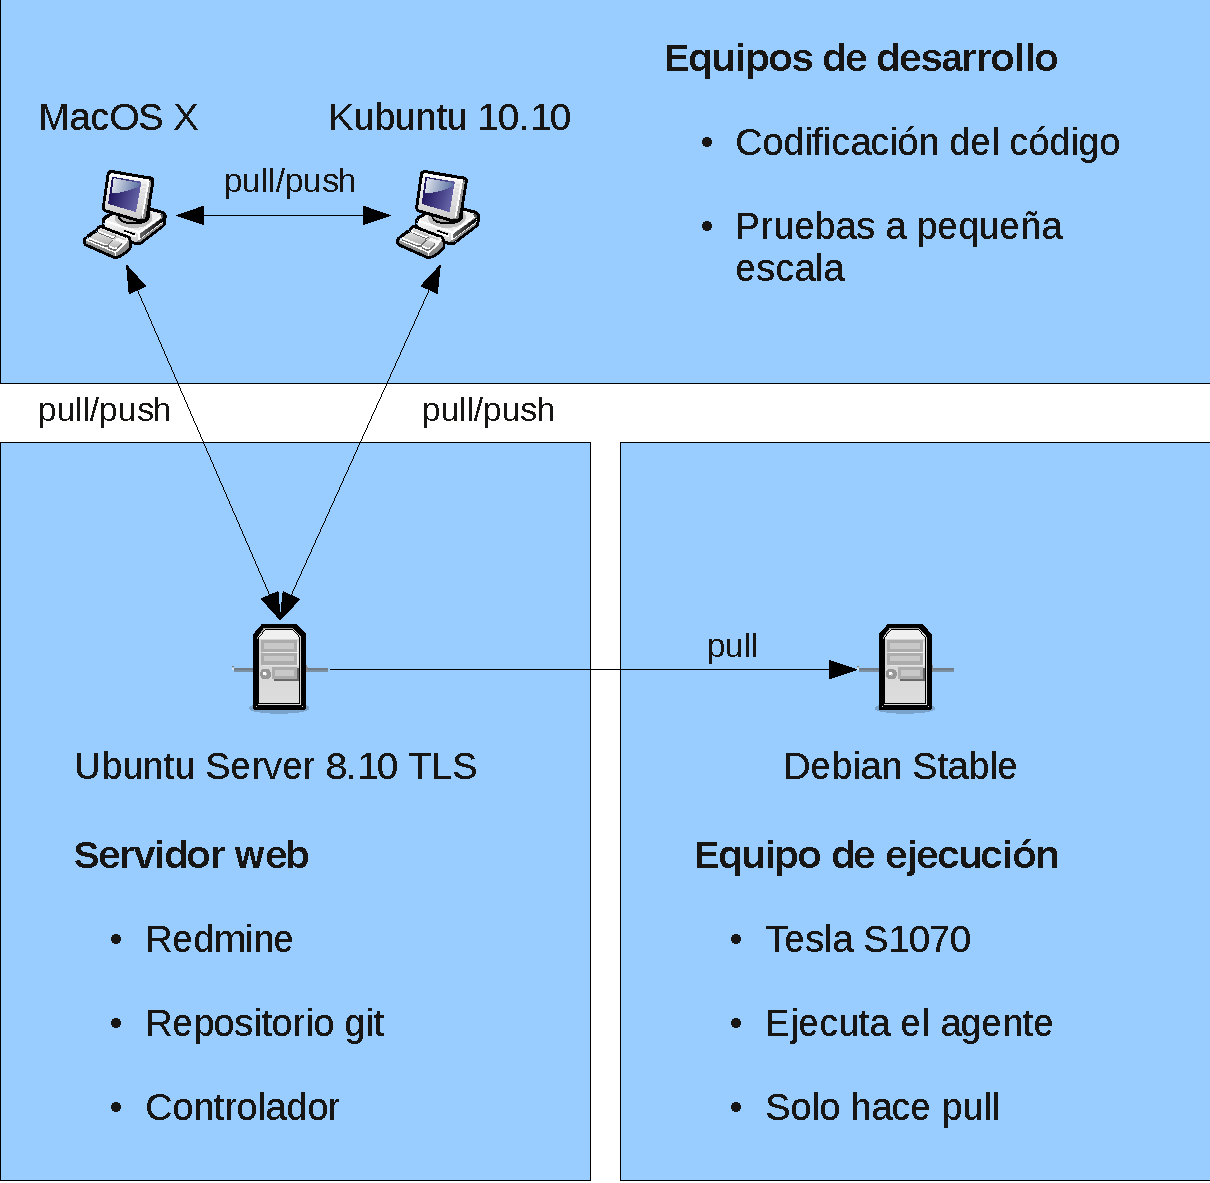
\includegraphics[width=0.7\textwidth]{images/entorno_trabajo.pdf}
	\caption{Diagrama del entorno de trabajo}\label{fig:entorno_trabajo}
\end{figure}